%!TEX root = ../../Main.tex
\graphicspath{{Chapters/Indledning/}}
%-------------------------------------------------------------------------------

\section{Indledning}
Næsten alle danskere har nu til dags en mobil på sig som, som indeholder et bluetooth modul. Dette vil vi gerne udnytte til at kunne låse og åbne hoveddøren hos private personer. Dette betyder at forbrugeren aldrig skal tænke på at have nøgle med fra hjemmet, eller finde dem inden man kan lukke sig selv ind. 
Denne prototype BA-TA (Bluetooth anti-theft alarm) vil derfor kunne låse og låse op for en dør, alt efter om man med sin bluetooth enhed er i nærheden af døren. Hele systemet styres fra en samlet enhed, som kan integeres fra brugeren gennem en skærm og dertilhørende touch funktion. 

\begin{figure}[H]
	\centering
	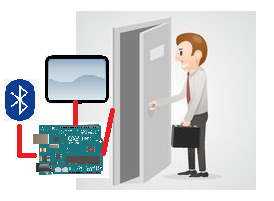
\includegraphics[width = 300 pt]{Img/Konceptbillede.png}
	\caption{Konceptbillede}
	\label{fig:Konceptbillede}
\end{figure}

Igennem brugergrænsefladen kan brugeren tilføje og fjerne enheder (personer) som skal kunne låse og låse op for døren. Når den sidste enhed er uden for rækkevidde, låses døren, og så snart systemet ser en godkendt enhed indenfor rækkevidden bliver døren låst op. 

